%% -------------------------------------------------------------------
%% Author    : Ashadul Halder; Soumik Ghosh
%%
%% To use the package fancymag, compilation must be done with lualatex 
%% and a few required folders (as outlined in the documentation) must be present 
%% in the working directory. These folders contain necessary font and style 
%% resources that the package depends on.
%% -------------------------------------------------------------------

\documentclass[10pt,twoside]{article}
\usepackage{xcolor}
\usepackage{lipsum}
\usepackage{fancymag} % Load the custom package
\usepackage[colorlinks=true, linkcolor=blue, urlcolor=cyan, citecolor=red]{hyperref}
\usepackage[most]{tcolorbox}
\usepackage{multicol}
\usepackage{enumitem}
\usepackage{float}
\usepackage{array}
\definecolor{accent}{HTML}{0080EE}
\begin{document}
	\sloppy
	
%%%%%%%%%%%%%%%%%%%%%  Cover page  %%%%%%%%%%%%%%%%%%%%%%%%%
    \begin{fistpg}
    	\begin{tikzpicture}[remember picture, overlay]
    		\node[anchor=south west, inner sep=0] at (current page.south west) {
    			
\includegraphics[width=\paperwidth, height=\paperheight]{img/fancymag-front.jpg}
    		};
    	\end{tikzpicture}
        \cleardoublepage
    \end{fistpg}
    
%%%%%%%%%%%%%%%%%%%%%  Inner page 1  %%%%%%%%%%%%%%%%%%%%%%%%%
	\begin{fistpg}
		\begin{tikzpicture}[remember picture, overlay]
			\node[anchor=south west, inner sep=0] at (current page.south west) {
				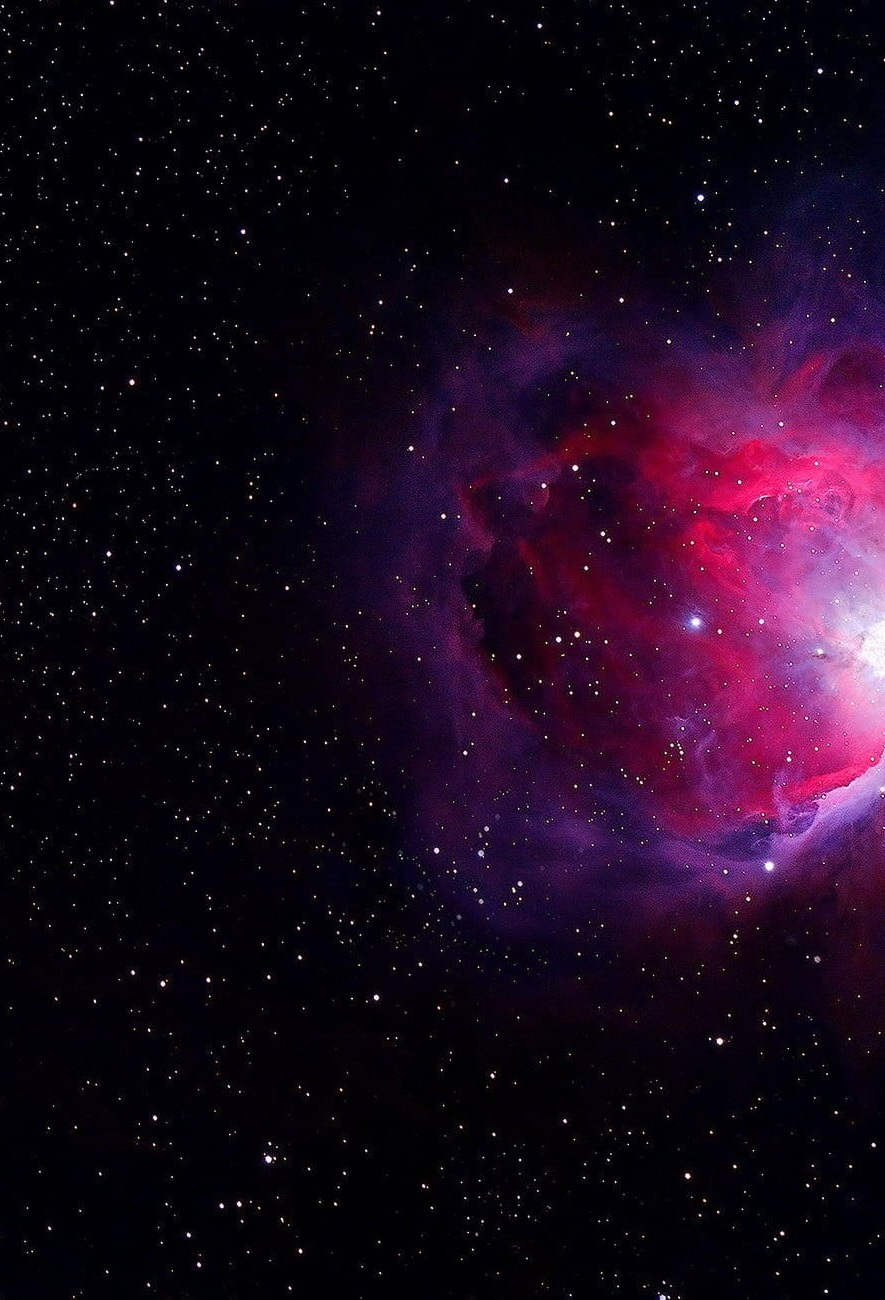
\includegraphics[width=\paperwidth, height=\paperheight]{img/fancymag-about_bg_1.jpg}
			};
		\end{tikzpicture}
		\begin{minipage}[l][\textheight]{0.65\textwidth}
			\begin{center}
				{\fontsize{20}{20} \selectfont \customfontone{\textcolor{cyan}{Title}}}\\
				{\fontsize{13}{13} \selectfont \customfontfour{\textcolor{white}{VOLUME XVII\\ (2025)}}}\\
				\vspace{0.5cm}
			\end{center}
			
			\begin{tcolorbox}[colback=blue!20!white, width=\textwidth, opacityfill=0.2]
				\textcolor{white}{\textbf{\lettrine{L}{}\lipsum[1-2]}}
			\end{tcolorbox}
		\end{minipage}
	\end{fistpg}
	
%%%%%%%%%%%%%%%%%%%%%  Inner page 2  %%%%%%%%%%%%%%%%%%%%%%%%%
		\begin{fistpg}
		\begin{tikzpicture}[remember picture, overlay]
			\node[anchor=south west, inner sep=0] at (current page.south west) {
				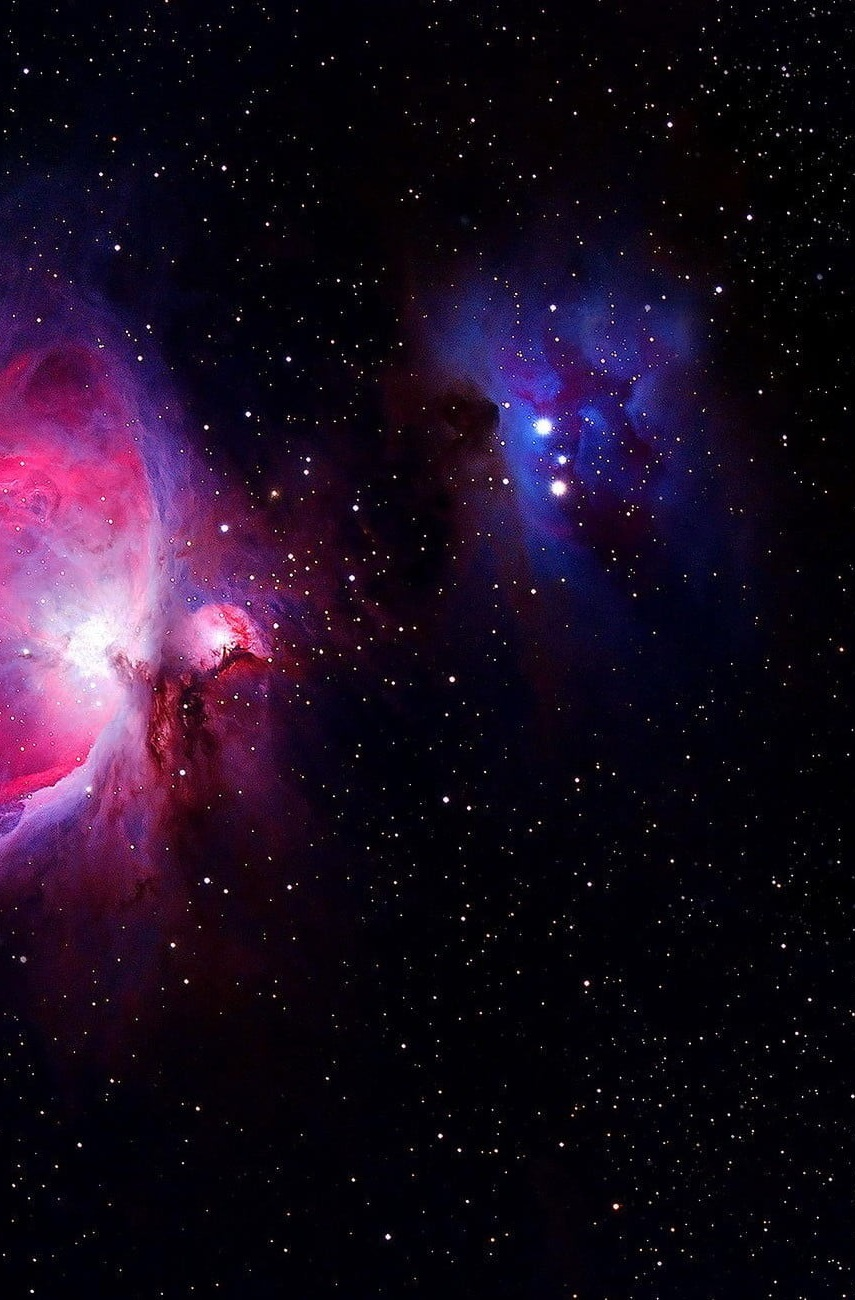
\includegraphics[width=\paperwidth, height=\paperheight]{img/fancymag-about_bg_2.jpg}
			};
		\end{tikzpicture}
		\begin{center}
			\vskip 3cm
			\begin{center}
				{
\includegraphics[height=3.5cm]{img/fancymag-logo.png}}\\
				\vspace{1cm}
				{\fontsize{60}{60} \selectfont \customfontone{\textcolor{white}{FANCYMAG}}}\\
				\vspace{1cm}
				{\fontsize{20}{20} \selectfont \customfontthree{\textcolor{cyan}{VERSION\\ (1.0)}}}\\
				\vspace{0.5cm}
			\end{center}
		\end{center}
	\end{fistpg}

%%%%%%%%%%%%%%%%%%%%%%%%%%%%%%%%%%%%%%%%%%%%%%%%%%%%%%%
{\bgchange{img/fancymag-bg_all.jpg}
    \newpage
    \begin{fistpg}
    	\vskip 1cm
    	\cleardoublepage
    \end{fistpg}
    \bgchange{img/fancymag-bg_all.jpg}
    \setcounter{page}{1}

%%%%%%%%%%%%%%%%%%%%% Messege %%%%%%%%%%%%%%%%%%%%%%%%%  
    \msg{Someone}{Designation}{Message from that person}{Affiliation}{img/fancymag-msg.png}{img/fancymag-m_sig.png}{3.5cm}{
    	\lettrine{T}{}he  \texttt{\textbackslash msg} command is a custom LaTeX macro defined in the \texttt{mag.sty} package. It is designed to format and display figures in a structured manner, placing them either to the left or right depending on the page type. This command helps maintain consistency in figure placement throughout a document.\\    	
    	The  \texttt{\textbackslash msg} command takes eight arguments and follows the syntax:\\
    	\texttt{\textbackslash msg\{arg1\}\{arg2\}\{arg3\}\{arg4\}\{arg5\}\{arg6\}\{arg7\}\{arg8\}}\\
    	Here, \texttt{arg1} and \texttt{arg2} typically define the figure source and description, while \texttt{arg4} through \texttt{arg7} control its size, alignment, and labeling. Arguments \texttt{arg3} and \texttt{arg8} may have specific uses depending on the document's requirements.\\
    	One key feature of  \texttt{\textbackslash msg} is its ability to adjust figure placement based on whether the current page is odd or even. Internally, the command calls \texttt{\textbackslash msgfigurer} for odd-numbered pages, aligning figures to the right, and \texttt{\textbackslash msgfigurel} for even-numbered pages, aligning figures to the left. This ensures that figures always appear near the outer margin, enhancing readability in two-sided documents.\\
    	A sample implementation using the  \texttt{\textbackslash msg} command might look like this:\\
    	\texttt{\textbackslash msg\{Figure1\}\{Description\}\{Unused\}\{0.5\}\{Center\}\{Scale\}\{Label\}\{Extra\}}\\
    	This structure allows the document to dynamically format figures based on the page number, making it a useful tool for professional reports and books.\\
    	To use  \texttt{\textbackslash msg}, ensure that \texttt{mag.sty} is included in your LaTeX project. Since some arguments may be ignored depending on the internal logic, refer to additional package documentation for precise customization. The ability to vary figure placement with page parity makes this command particularly useful for creating well-structured, visually appealing documents.}
    
    \msg{Someone else}{Designation}{Message from another person}{Affiliation}{img/fancymag-msg1.png}{img/fancymag-m_sig.png}{3.5cm}{
    	\lettrine{H}{}ere \texttt{\textbackslash msg} is used to show the change of design with page number (odd to even or vice-versa)}
    
%%%%%%%%%%%%%%%%%%%%% Other Detail %%%%%%%%%%%%%%%%%%%%%%%%% 
  	\newpage
  	\fancyhead[LO]{\textcolor{accent}{\large\textbf{Fancymag}}}
  	\fancyhead[RE]{\textcolor{accent}{\large\textbf{Fancymag}}}
  	\fancyhead[RO]{\textcolor{accent}{\large\textbf{\thepage}}}
  	\fancyhead[LE]{\textcolor{accent}{\large\textbf{\thepage}}}
  	
  	{\fontsize{15}{15}\selectfont \textbf{\textcolor{accent}{\textsf{{Font Availability Note}}}}}\\
  	
\begin{tikzpicture}
  		\draw[fill={rgb,1:red,0;green,0;blue,0.7}, draw=none] (0, 0) rectangle (5cm, 0.15cm);
  	\end{tikzpicture}
  	\vskip 0.4cm
  		\albumphoto{Font Availability Note}{2024}{img/fancymag-di.png}
  	 	\section*{Font Availability Note}
  	 	This package requires LuaLaTeX and uses fonts bundled locally in the \texttt{fonts/} folder. These fonts are not installed system-wide and TeX distributions like TeX Live or MiKTeX may not provide them automatically. Users must compile their documents in the same directory as the \texttt{fonts/} folder.
  	 	\\
  	 	\begin{tcolorbox}[colback=blue!5!white, width=\textwidth, opacityfill=0.1]
  	 		{\fontsize{14}{14}\selectfont {Custom fonts}}\\
  	 		\begin{tabular}{l m{10cm}}
  	 			\textbf{Command Name} & \textbf{Example Output} \\
  	 			\hline\\
  	 			\textbackslash customfontone & {\customfontone The quick brown fox jumps over the lazy dog.} \\
  	 			\textbackslash customfonttwo & {\customfonttwo The quick brown fox jumps over the lazy dog.} \\
  	 			\textbackslash customfontthree & {\customfontthree The quick brown fox jumps over the lazy dog.} \\
  	 			\textbackslash customfontfour & {\customfontfour The quick brown fox jumps over the lazy dog.} \\
  	 			\textbackslash headrf & {\headrf The quick brown fox jumps over the lazy dog.} \\
  	 		\end{tabular}
  	 		
  	 	\end{tcolorbox}
  	% ________________________
  	 	\newpage
  	 	{\fontsize{15}{15}\selectfont \textbf{\textcolor{accent}{\textsf{{Important notes}}}}}\\
  	 	\bullet Don't remove the `fancymag-msg\_bg.jpg' and `fancymag-blank.png' from the \texttt{img} folder.\\
  	 	\bullet Don't remove any font from the \texttt{font} folder.\\
  	 	\bullet Use LuaLaTeX to compile.\\
  	 	\bullet The \texttt{fancymag.sty} file, along with the \texttt{img/} and \texttt{fonts/} folders, must be placed in the same directory as the main \texttt{.tex} file that uses this package. This ensures that all local resources — such as custom fonts and profile images — are correctly located by the package using relative paths via \texttt{fontspec} and \texttt{graphicx}.
  	 	
  	 	The recommended directory structure is as follows:
  	 	
  	 	\begin{verbatim}
  	 		project/
  	 		├── mainfile.tex       % Your main document
  	 		├── fancymag.sty       % The package file
  	 		├── mainfile.pdf       % Compiled documentation (optional)
  	 		├── fonts/             % Folder containing .ttf font files
  	 		│   ├── Audiowide-Regular.ttf
  	 		│   └── ...
  	 		├── img/               % Folder containing image assets
  	 		│   ├── msg1.png
  	 		│   └── ...
  	 	\end{verbatim}


%%%%%%%%%%%%%%%%%%%%% Interview %%%%%%%%%%%%%%%%%%%%%%%%% 
  \titlepg{Interview}
 
  \interview{Dr. A}{Designation} {From:}{Institute}{Alumnus}{Department}{Institute}{img/fancymag-msg1.png}{
  		The \texttt{\textbackslash interview} command provides a structured and visually appealing layout for typesetting interviews in academic or editorial publications. It displays the interviewee's name, designation, affiliations and an image, followed by the interview content.\\
  		the syntax is \\
  		\texttt{\textbackslash interview{<Name>}{<Designation>}{<Label1:>}{<Affiliation1>}{<Label2:>}{<Affiliation2>}\\{<ImagePath>}{<Interview Content>}}\\
  		$\bullet$ \textbf{Name} - Name of the interviewee (e.g., \texttt{Dr. A})\\
  		$\bullet$ \textbf{Designation} - Title or position (e.g., \texttt{Senior Scientist})\\
  		$\bullet$ \textbf{Label1} - Label for first affiliation\\
  		$\bullet$ \textbf{Affiliation1} - First institution or organization\\
  		$\bullet$ \textbf{Label2} - Second label\\
  		$\bullet$ \textbf{Affiliation2} - Second institution or department\\
  		$\bullet$ \textbf{ImagePath} - Path to the interviewee's photo (e.g., \texttt{fancymag-msg1.png})\\
  		$\bullet$ \textbf{Interview Content} - The body of the interview, which can include paragraphs, formatting and styled text.\\
  		\noindent This command is designed for use with \textbf{LuaLaTeX}. Ensure that the image path is correct relative to your `.tex' file and that the required fonts and colors (e.g., \texttt{mt}) are defined in your document or the package.
  		
  		\begin{flushright}
  			\large{\textbf{Someone}}\\
  			\textcolor{mt}{\textit{Some text}}
  		\end{flushright}
  		}
  	

%%%%%%%%%%%%%%%%%%%%% Article Type 1 %%%%%%%%%%%%%%%%%%%%%%%%% 
  \titlepg{Article Type 1}
  
  	\begin{particle1}{Particle 1}{detail 1}{Name}{detail 2}{detail 3}{detail 4}{img/fancymag-msg.png}
  	{It is Abstract}  	
  	{\lettrine{T}{}he \texttt{particle1} environment is a custom LaTeX construct used to create a stylized profile or informational block. It accepts nine arguments, which include textual information, an image path, an abstract and a main body of content. This environment is suitable for formatting personal profiles, author introductions, interview or structured descriptions in a visually engaging format.\\
  	The syntax is as follows:\\
  	\texttt{\textbackslash begin\{particle1\}\{Title\}\{Detail 1\}\{Name\}\\\{Detail 2\}\{Detail 3\}\{Detail 4\}\{img.png\}\\\{Abstract\}\{Main Text\}\\\textbackslash end\{particle1\}}\\
  	\bullet \textbf{The first argument}, \texttt{Title}, is used as the main heading or role, such as ``Professor" or ``Lead Scientist".\\
  	\bullet \textbf{The second argument}, \texttt{Detail 1}, typically describes a category or department, such as ``Astrophysics Division".\\
  	\bullet \textbf{The third argument}, \texttt{Name}, is the full name of the person being described.\\  	
  	\bullet \textbf{ The fourth, fifth, and sixth arguments} - \texttt{Detail 2}, \texttt{Detail 3}, and \texttt{Detail 4} — are additional attributes or information related to the subject, such as degrees, research areas, affiliations, achievements, or roles.\\  	
  	\bullet \textbf{The seventh argument} is the image path, such as \texttt{img/fancymag-author.png}, pointing to a profile picture or representative image that will be displayed alongside the text.\\  	
  	\bullet \textbf{The eighth argument} is an abstract or summary sentence that concisely describes the subject's main role, focus, or expertise. It serves as a short introduction or tagline.\\  	
  	\bullet \textbf{The ninth and final argument} is the main body text. This is a longer paragraph or content block that provides a detailed explanation or narrative about the subject.}  		
  	\end{particle1}
  	
	\begin{particle1}{Particle 1}{detail 1}{Name}{detail 2}{detail 3}{detail 4}{img/fancymag-msg1.png}
	{It is Abstract}
	{\textbf{Note:} The visual layout of the \texttt{particle1} environment may depend on whether it appears on an \textbf{odd} or \textbf{even} page. In many designs, the placement of the image and text is reversed or mirrored to maintain symmetry in double-sided documents. This behavior is typically implemented using conditional checks within the environment's definition. As a result, the final appearance may vary depending on the page number where the environment is placed.}
  	\end{particle1}
  
%%%%%%%%%%%%%%%%%%%%% Article Type 2 %%%%%%%%%%%%%%%%%%%%%%%%%   
  \titlepg{Article Type 2}

    \begin{particle2}{Title}{Author}{Detail 1}{Detail 2} {img/fancymag-msg.png}{img/fancymag-side.jpeg}
                
        The \texttt{particle2} environment is a custom LaTeX, which is well-suited for article-style entries, research summaries, or section headers that include detailed narrative text and embedded visuals.
        
        The syntax is as follows:
        
        \texttt{\textbackslash begin\{particle2\}\{Title\}\{Author\}\{Detail 1\}\{Detail 2\}\{author.png\}\{side.jpeg\}}\\
        \texttt{Body text (including paragraphs, figures, etc.)}\\
        \texttt{\textbackslash end\{particle2\}}
        
        This environment takes six arguments before the body content begins. These arguments are used to build a structured header or banner area before rendering the main text.
        
        The arguments are:
        
        \bullet \textbf{Title} – The title or heading of the section, often representing a topic or article name.
        
        \bullet \textbf{Author} – The name of the author or contributor for this content block.
        
        \bullet \textbf{Detail 1} – A short detail such as a role, subtitle, or classification label.
        
        \bullet \textbf{Detail 2} – Another short descriptor, for example, affiliation or focus area.
        
        \bullet \textbf{msg.png} – The primary image, typically used as a profile photo or symbolic image, placed near the title and author.
        
        \bullet \textbf{side.jpeg} – A secondary image which appears as sidebar  background for the first page only.
        
    \end{particle2}
    
    \begin{particle2}{Title}{Author}{Detail 1}{Detail 2} {img/fancymag-msg.png}{img/fancymag-di1.png}
    	
		\textbf{Note:} The visual layout of the \texttt{particle2} environment may depend on whether it appears on an \textbf{odd} or \textbf{even} page. In many designs, the placement of the image and text is reversed or mirrored to maintain symmetry in double-sided documents. This behavior is typically implemented using conditional checks within the environment's definition. As a result, the final appearance may vary depending on the page number where the environment is placed.
    	
    \end{particle2}

         
%%%%%%%%%%%%%%%%%%%%% Photographs and Paintings %%%%%%%%%%%%%%%%%%%%%%%%%   
  \titlepg{Paintings}

  	\fancyhf{}
  	\fancyhead[LO]{\textcolor{accent}{\large\textbf{Paintings}}}
  	\fancyhead[RE]{\textcolor{accent}{\large\textbf{Paintings}}}
  	\fancyhead[RO]{\textcolor{accent}{\large\textbf{\thepage}}}
  	\fancyhead[LE]{\textcolor{accent}{\large\textbf{\thepage}}}
  	
  	\photograph{Person 1}{Portrait, Left aligned}{Detail 2}{Detail 2}{img/fancymag-di1.png}{portrait}{left}
  	
  	\photograph{Person 2}{Portrait, Right aligned}{Detail 2}{Detail 2}{img/fancymag-di1.png}{portrait}{right}
  	
  	\photograph{Person 3}{Landscape, Right aligned}{Detail 2}{Detail 2}{img/fancymag-di.png}{landscape}{right}
  	
  	\photograph{Person 4}{Landscape, Left aligned}{Detail 2}{Detail 2}{img/fancymag-di.png}{landscape}{left}
  	
%%%%%%%%%%%%%%%%%%%%% Last page %%%%%%%%%%%%%%%%%%%%%%%%%  
	\newpage
	 \begin{fistpg}
		\begin{tikzpicture}[remember picture, overlay]
			\node[anchor=south west, inner sep=0] at (current page.south west) {
				
\includegraphics[width=\paperwidth, height=\paperheight]{img/fancymag-back.jpg}
			};
		\end{tikzpicture}
		\clearpage
	\end{fistpg}
\end{document}